\section{am::lambda::pf\_\-memdata$<$ P, O, U $>$ Struct Template Reference}
\label{structam_1_1lambda_1_1pf__memdata}\index{am::lambda::pf_memdata@{am::lambda::pf\_\-memdata}}
{\tt \#include $<$lambda.hpp$>$}

Inherits {\bf am::lambda::detail::lambda\_\-op\_\-tag}.

Inheritance diagram for am::lambda::pf\_\-memdata$<$ P, O, U $>$:\begin{figure}[H]
\begin{center}
\leavevmode
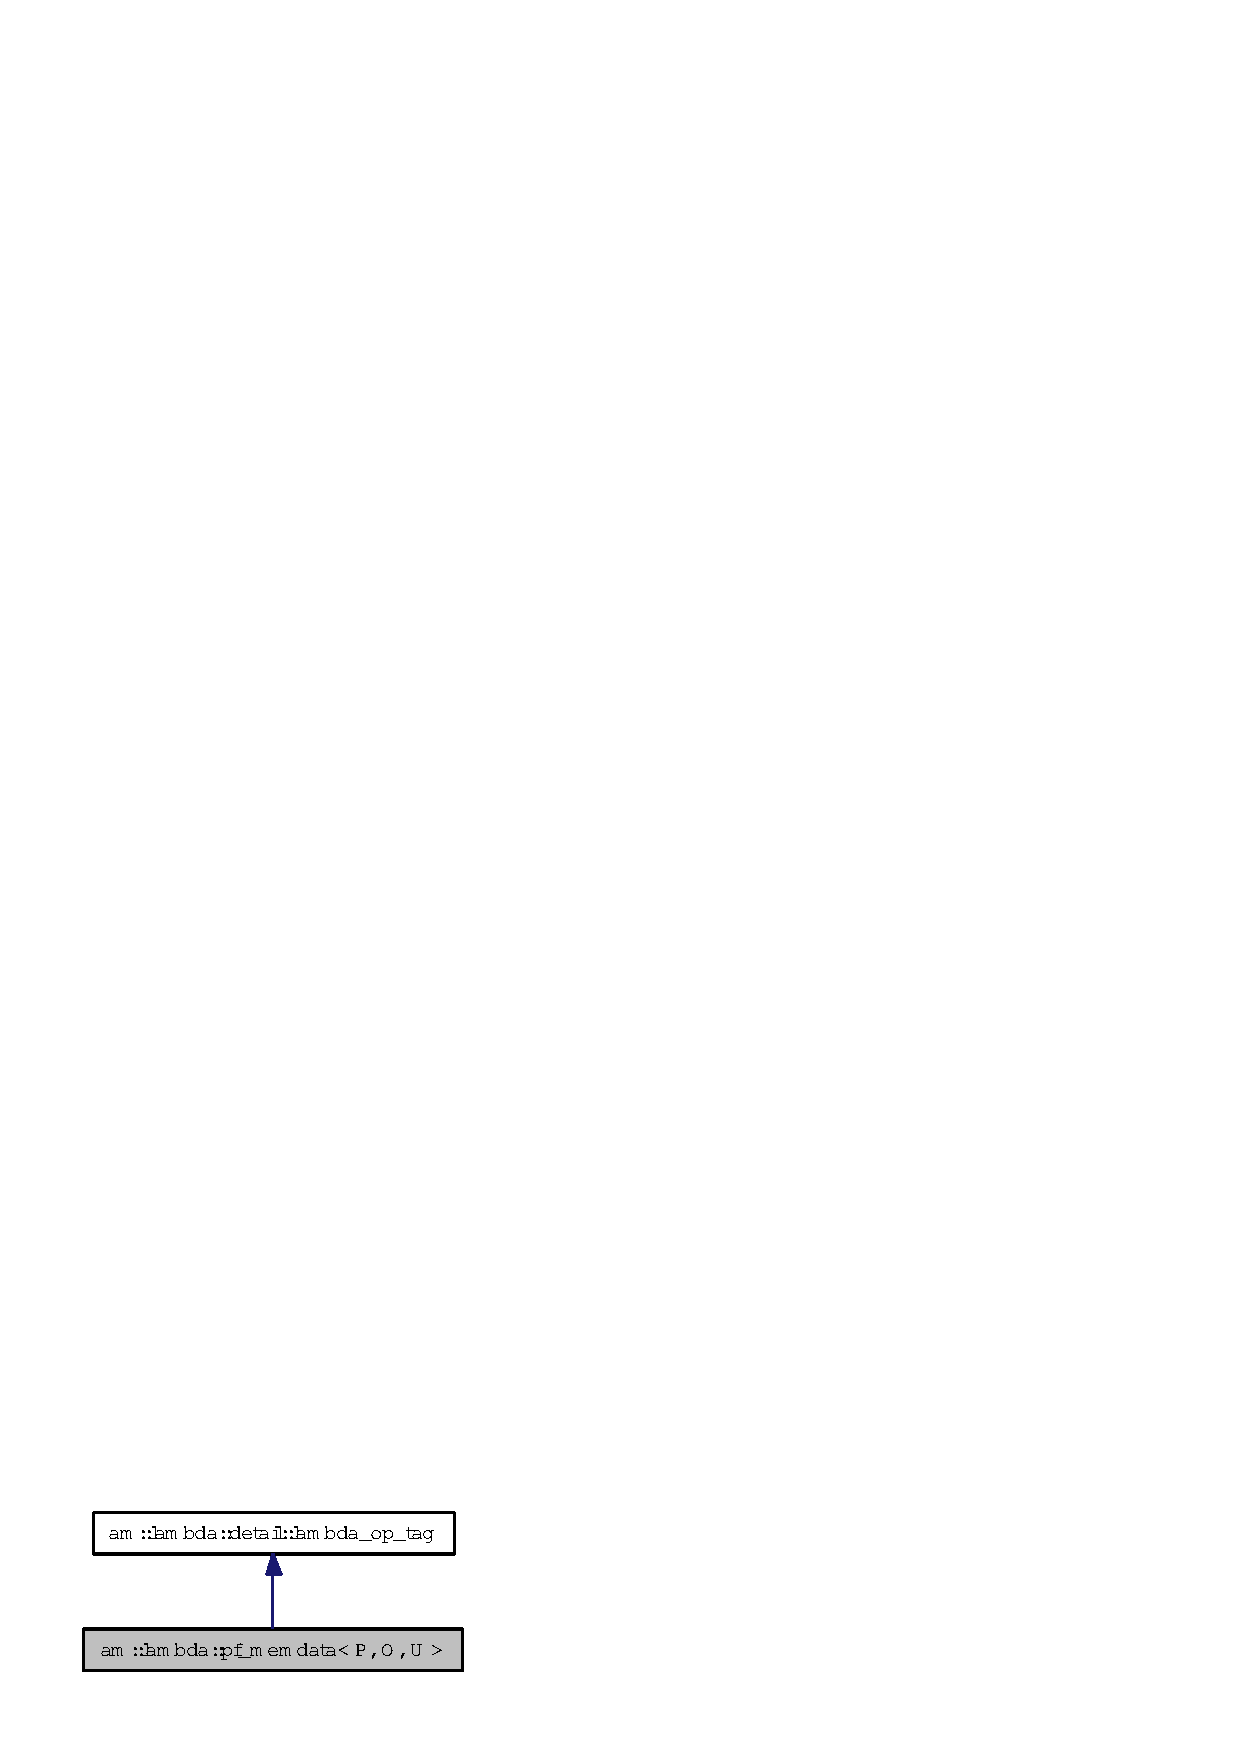
\includegraphics[width=113pt]{structam_1_1lambda_1_1pf__memdata__inherit__graph}
\end{center}
\end{figure}
Collaboration diagram for am::lambda::pf\_\-memdata$<$ P, O, U $>$:\begin{figure}[H]
\begin{center}
\leavevmode
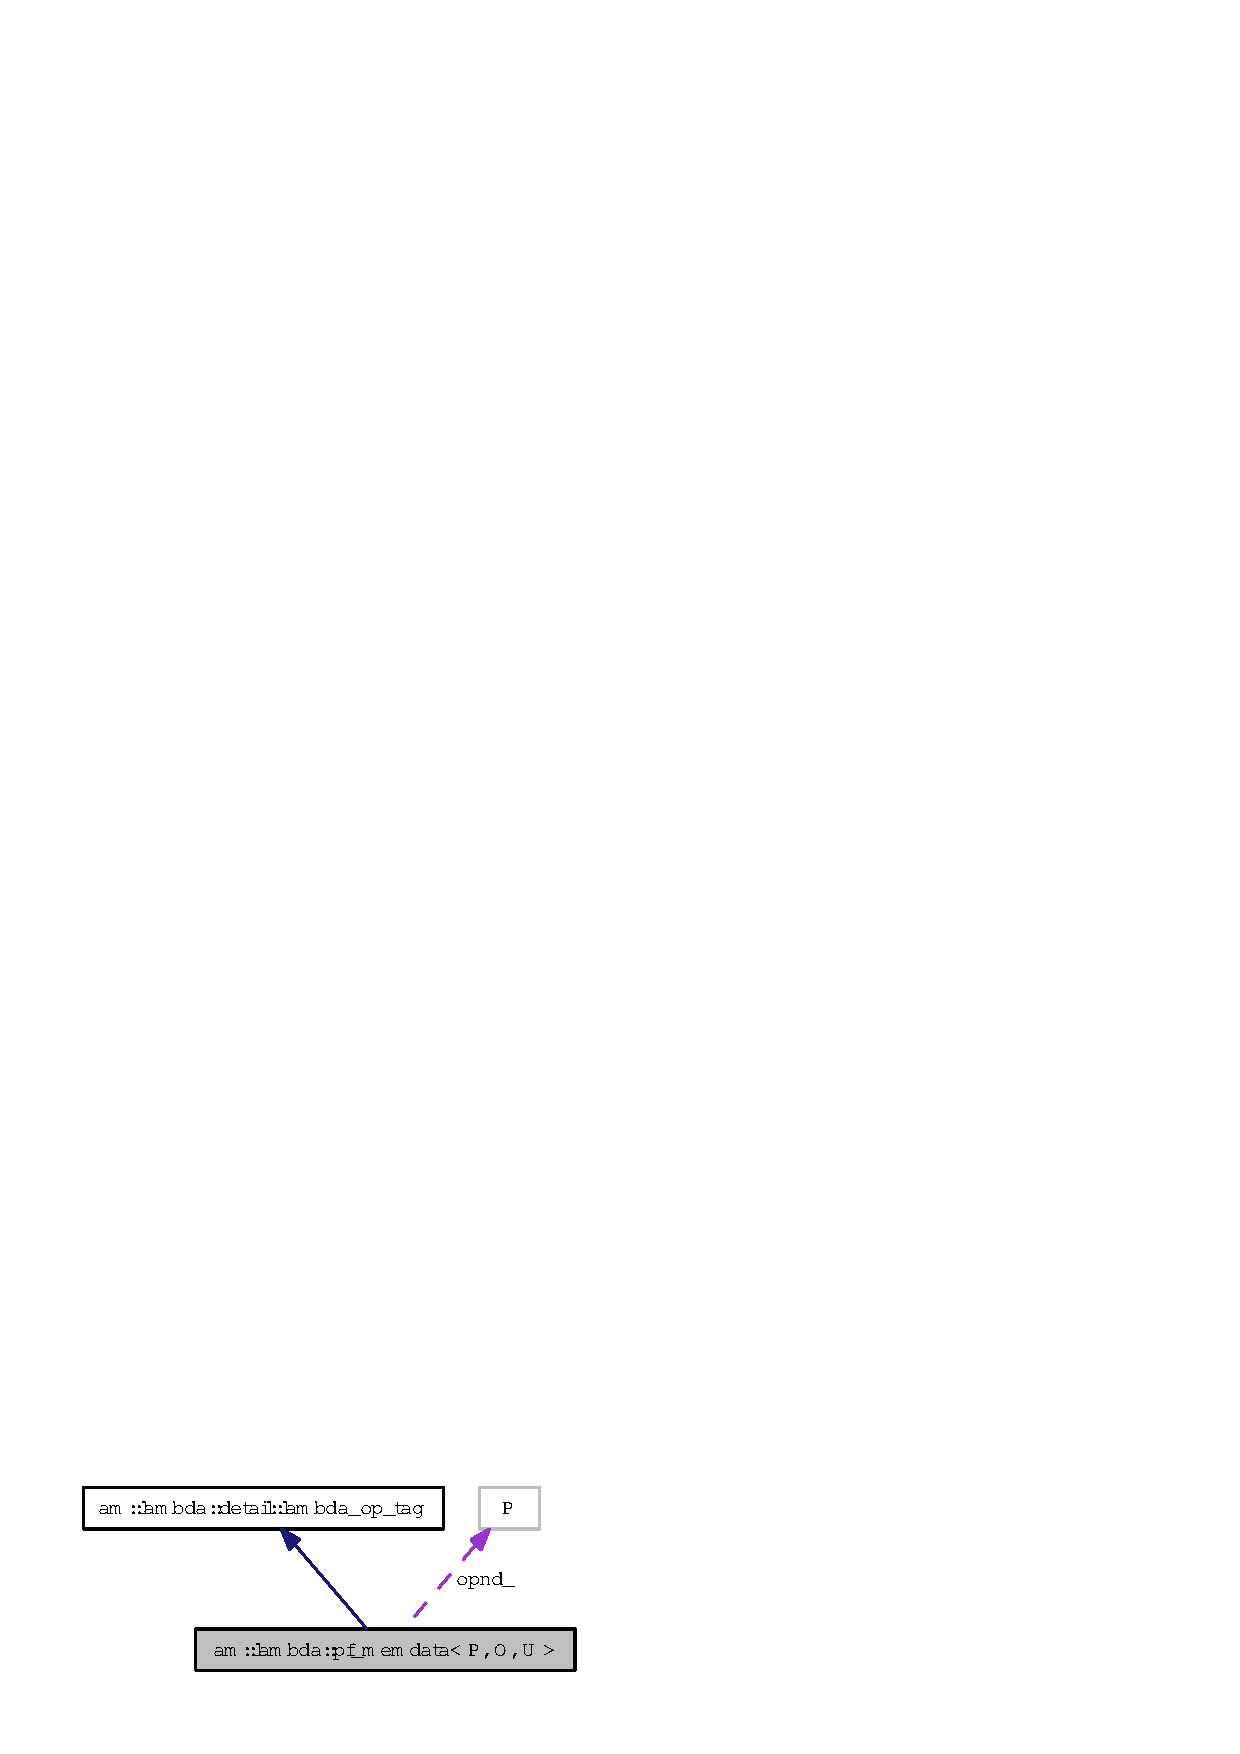
\includegraphics[width=140pt]{structam_1_1lambda_1_1pf__memdata__coll__graph}
\end{center}
\end{figure}
\subsection*{Public Member Functions}
\begin{CompactItemize}
\item 
\textbf{pf\_\-memdata} (P opnd, U(O::$\ast$pu))\label{structam_1_1lambda_1_1pf__memdata_9fe96a12a227ed71cc1b0726116c8fb3}

\item 
template$<$class T1, class T2, class T3$>$ U const \& \textbf{operator()} (T1 \&t1, T2 \&t2, T3 \&t3) const \label{structam_1_1lambda_1_1pf__memdata_b40e1eefad6d26a955ffb4cc82434650}

\item 
template$<$class T1, class T2$>$ U const \& \textbf{operator()} (T1 \&t1, T2 \&t2) const \label{structam_1_1lambda_1_1pf__memdata_c6274e3380a83ffe6b2d96e1a36ddb68}

\item 
template$<$class T1$>$ U const \& \textbf{operator()} (T1 \&t1) const\label{structam_1_1lambda_1_1pf__memdata_60d1c08701f9c711ce5cbf8b505e5efe}

\item 
{\bf address\_\-of} \textbf{operator \&} () const\label{structam_1_1lambda_1_1pf__memdata_860bb00118c6f6147c231a62eaa50fcd}

\end{CompactItemize}
\subsection*{Public Attributes}
\begin{CompactItemize}
\item 
P \textbf{opnd\_\-}\label{structam_1_1lambda_1_1pf__memdata_9cff67d816aefbe768f8d72ff882db4b}

\item 
UO::$\ast$ \textbf{pu\_\-}\label{structam_1_1lambda_1_1pf__memdata_a44cac02967ca15bd8efaa831454e5d6}

\end{CompactItemize}
\subsection*{Classes}
\begin{CompactItemize}
\item 
struct {\bf address\_\-of}
\end{CompactItemize}


\subsection{Detailed Description}
\subsubsection*{template$<$class P, class O, class U$>$ struct am::lambda::pf\_\-memdata$<$ P, O, U $>$}

\begin{Desc}
\item[For internal use only.]
Pure Function to support member data pointer access. \end{Desc}




The documentation for this struct was generated from the following file:\begin{CompactItemize}
\item 
{\bf lambda.hpp}\end{CompactItemize}
